\documentclass{beamer}
\renewcommand{\baselinestretch}{1.1}
\usepackage{graphicx}
\usepackage{natbib}
\usepackage{amsmath}
\usepackage{hyperref}
\usepackage{listings} 

\def\labelitemi{--}
\parindent=0pt

\usepackage{xcolor}

\colorlet{codecolor}{black!30}
\newcommand{\codebox}[1]{%
  \colorbox{codecolor}{\ttfamily \detokenize{#1}}%
}

\begin{document}


{\usebackgroundtemplate{%
  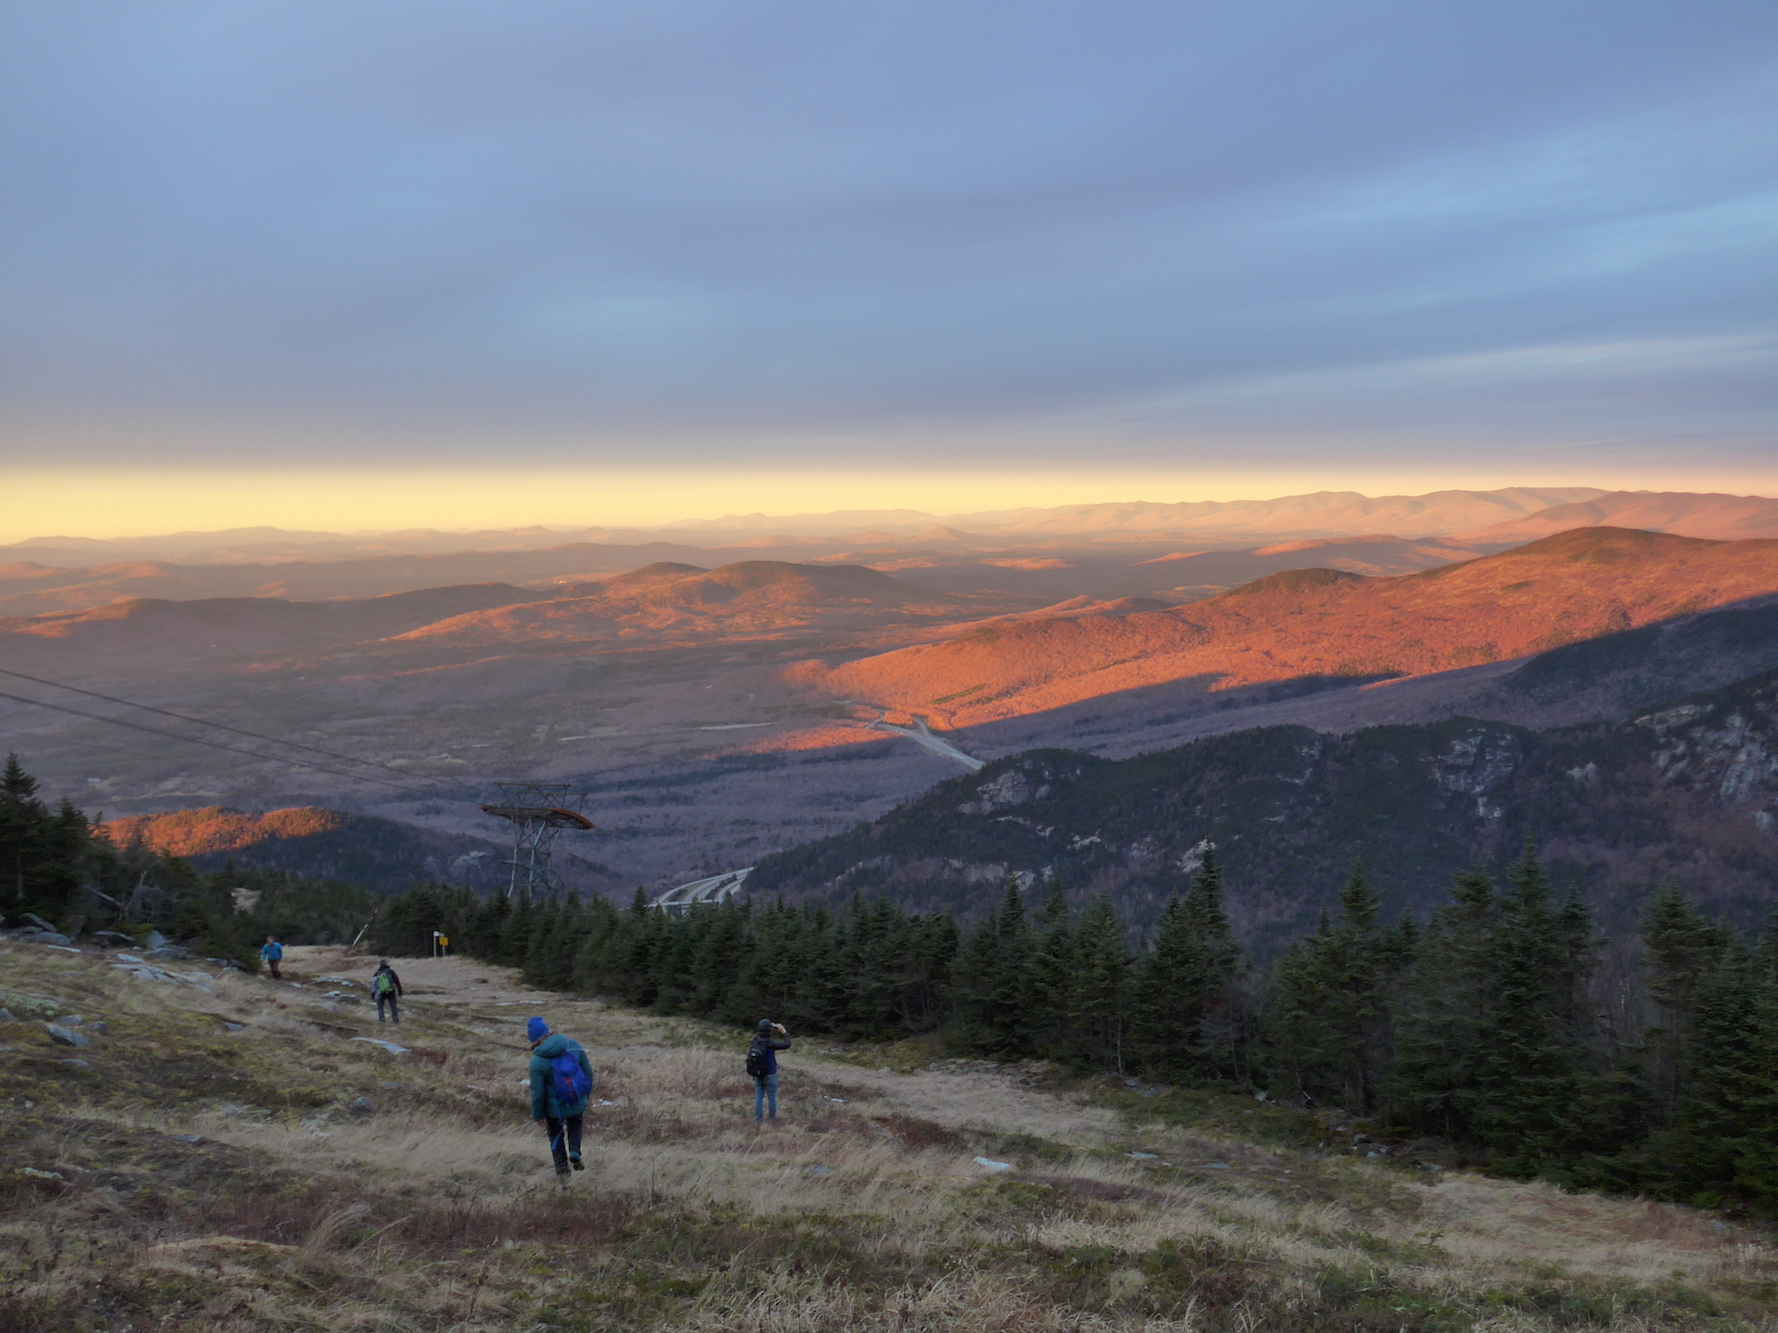
\includegraphics[width=\paperwidth,height=\paperheight]{2016Nov10_Cannon329sm.jpg}} 
\begin{frame}
\begin{center}
\vspace{5ex}
{\color{white} {\huge Rangers update}}
\\
\vspace{2ex}
{\color{white} {\Large 5 November 2020}}

\end{center}
\end{frame}
}
	
	\frame{
		\frametitle{Background}
		\framesubtitle{}
Why do species differ in cues?
\vspace{5ex}\\
Armed with species-level estimates of cue-use from our OSPREE database, grided climate data and species distribution maps, our team will range for to test this prediction.
	}

	\frame{
		\frametitle{Predictions... }
		\framesubtitle{}
		\begin{itemize}
			\item  If forcing (considered to be the primary cue) is an unreliable indicator of appropriate spring growing conditions, than species will rely more heavily on secondary cues. 
\item We also would expect that species must encounter the cue conditions (ie tropical species shouldn't have a chilling cue).

\item But what makes forcing unreliable? High inter and/ or intra-annual variability among locations or years. We think that the latter is more important, but a recent study boy Zohner found the former to matter.
		\end{itemize}
	}



	\frame{
		\frametitle{Side bar: temporal vs. geographic variability}
		\framesubtitle{}
% Inter-annual variability for a given grid cell, or variation among grid cells at a give time. We think that both kinds of variation could in theory drive selection for cue use if we assume cue use is relatively conserved within species.

\begin{figure}[h!]
    \centering
         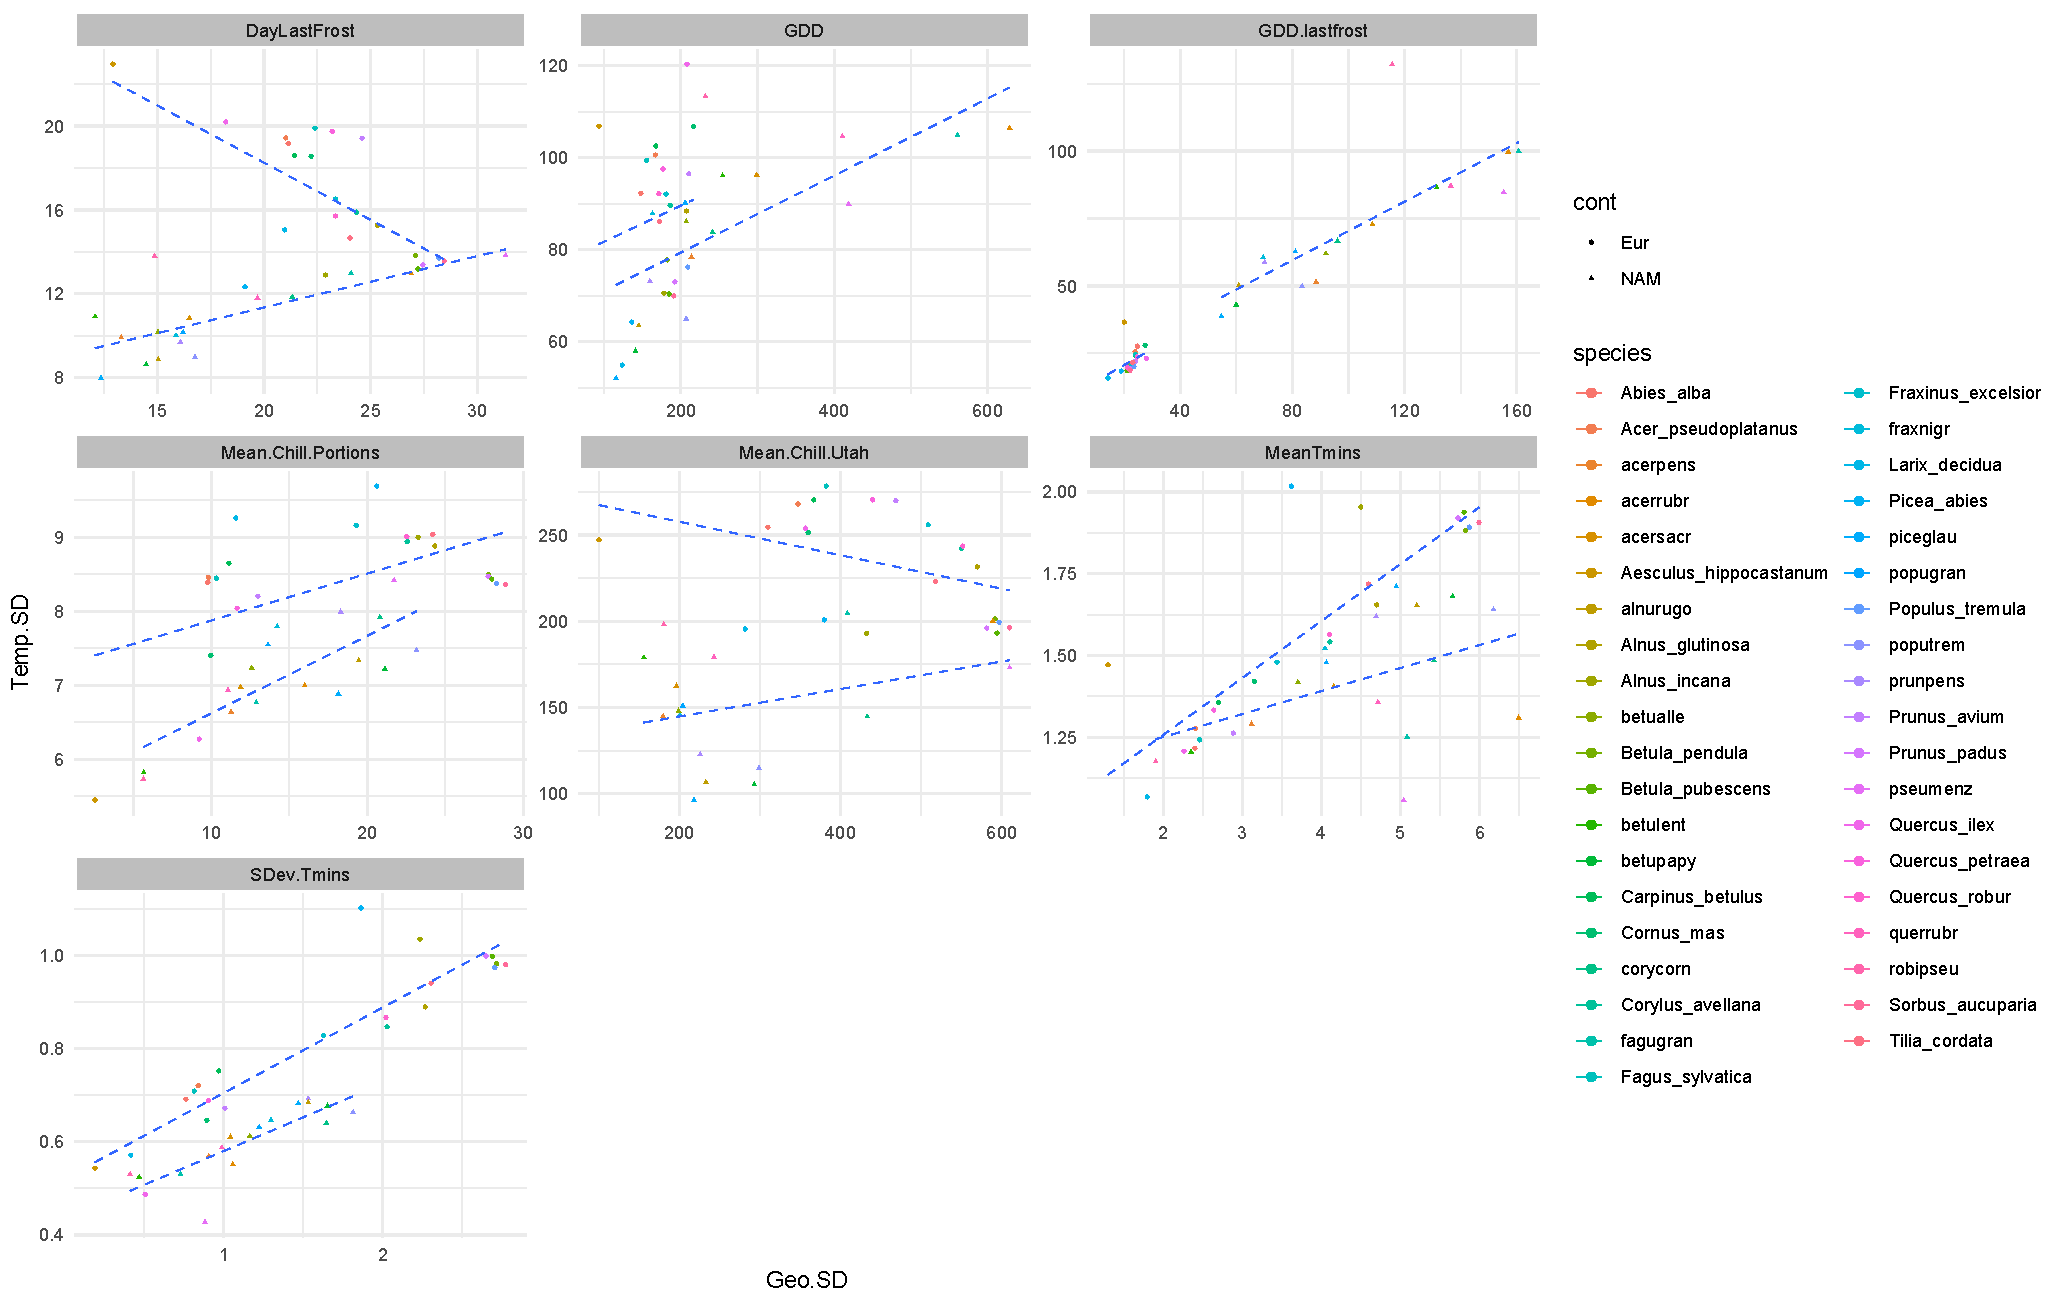
\includegraphics[width=0.9\textwidth]{..//..//figures/spatial_vs_temporal/spatialtemporal_sds.pdf}
    \caption{Correlation between temporal and geographic standard deviation of climate parameters} 
    \label{fig:tempgeo}
\end{figure}
	}



	\frame{
		\frametitle{Hypothesis 1}
		\framesubtitle{North America species (which experience a more variable spring environment) should have stronger photoperiod and chilling cue than European species}
\begin{figure}[h!]
    \centering
         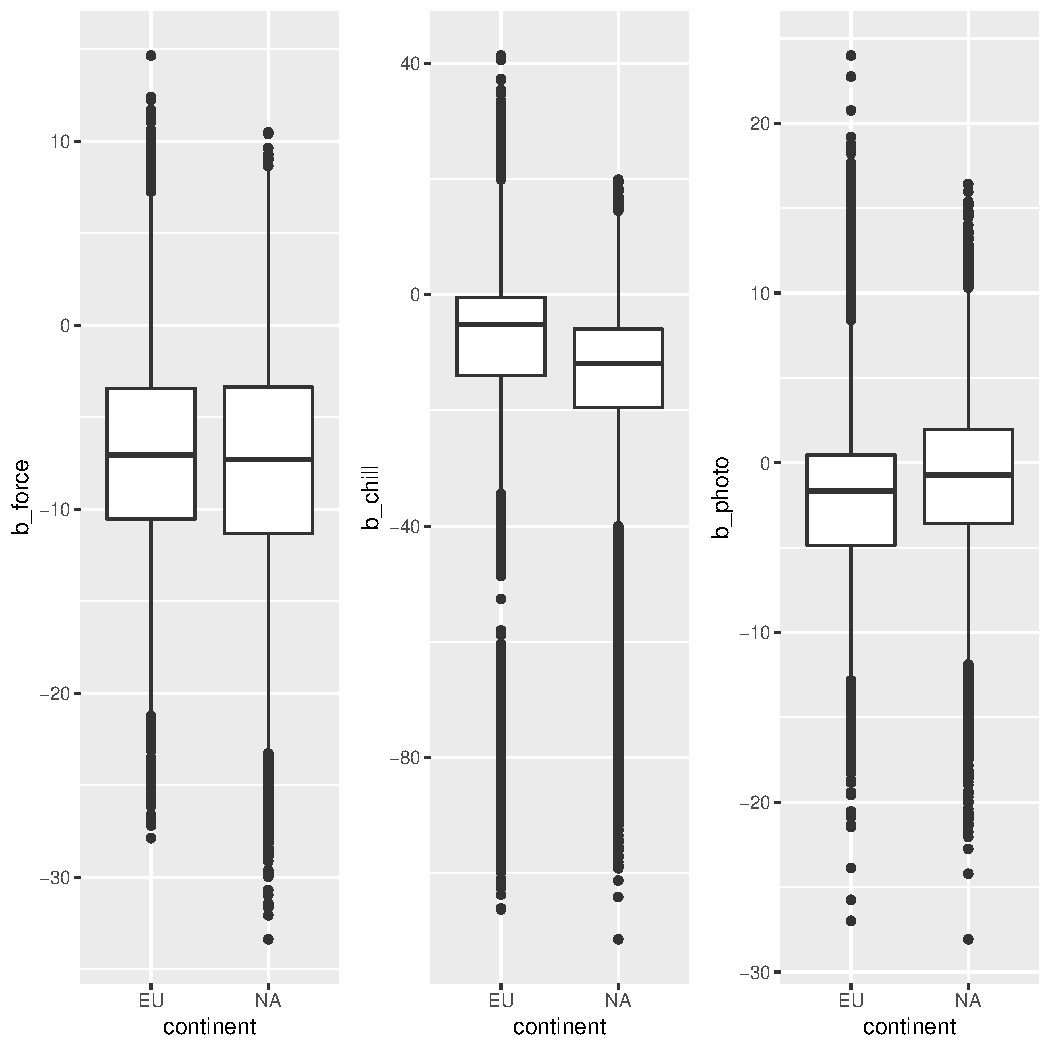
\includegraphics[width=0.5\textwidth]{..//..//figures/continental_cues.pdf}
    \caption{ Chilling and Photoperiod cues use is stronger (more negative) in North America} 
    \label{fig:continent}
\end{figure}

	}



	\frame{
		\frametitle{Hypothesis 2}
		\framesubtitle{Standard deviation of growing degree days until last frost should correlate with higher (more negative) chill sensitivity}
\begin{figure}[h!]
    \centering
         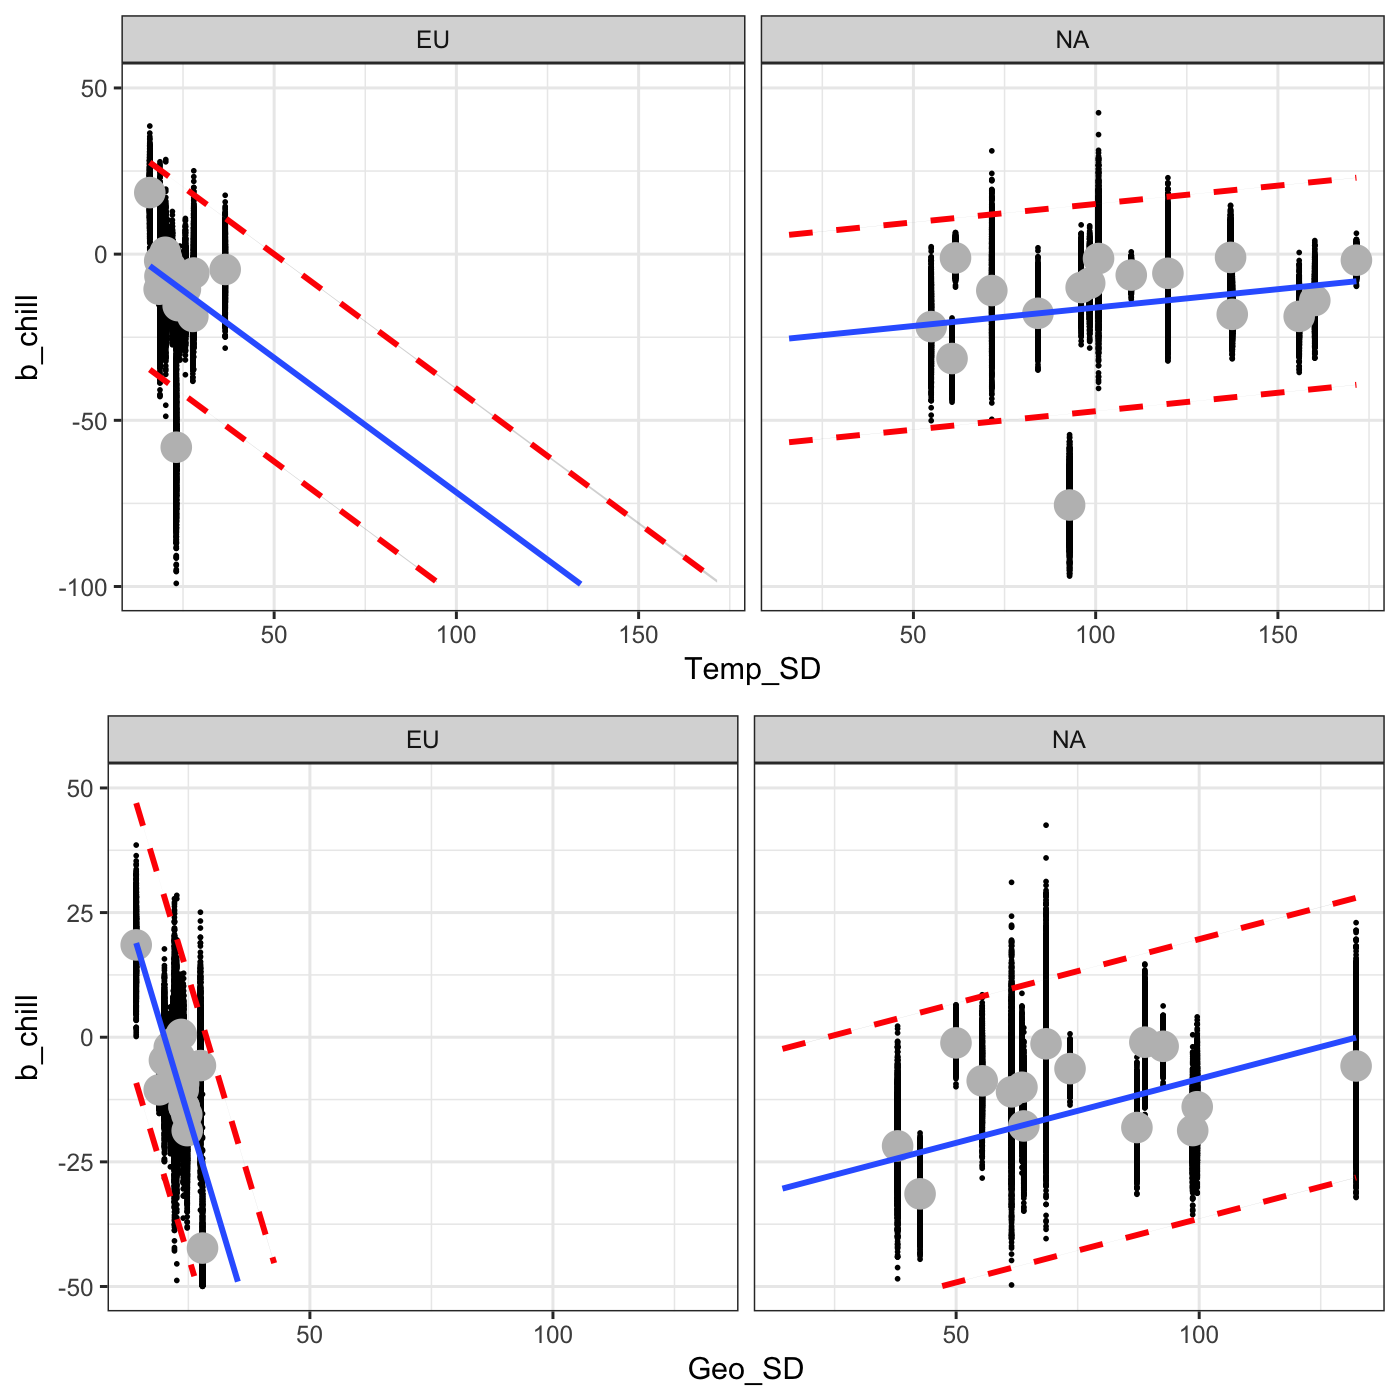
\includegraphics[width=0.5\textwidth]{..//..//figures/cheap_approach/modeled_gdd2lf.png}
    \caption{Influence of temporal and geographic variation in growing degrees to last frost on $\beta_{chill}$. Model is pooling on iterations. Blue line is mean and red lines 95\% credible intervals} 
    \label{fig:gddlf}
\end{figure}


	}


	\frame{
		\frametitle{Hypothesis 3}
		\framesubtitle{Standard deviation of mean winter temperatures (STV) should correlate with higher (more negative) chill sensitivity}
\footnotesize{This hypothesis was supported by Zohner's work. However, we think it might be an artifact of not explicitly including phenology into our models. Its also not supper supported in our data }
\begin{figure}[h!]
    \centering
         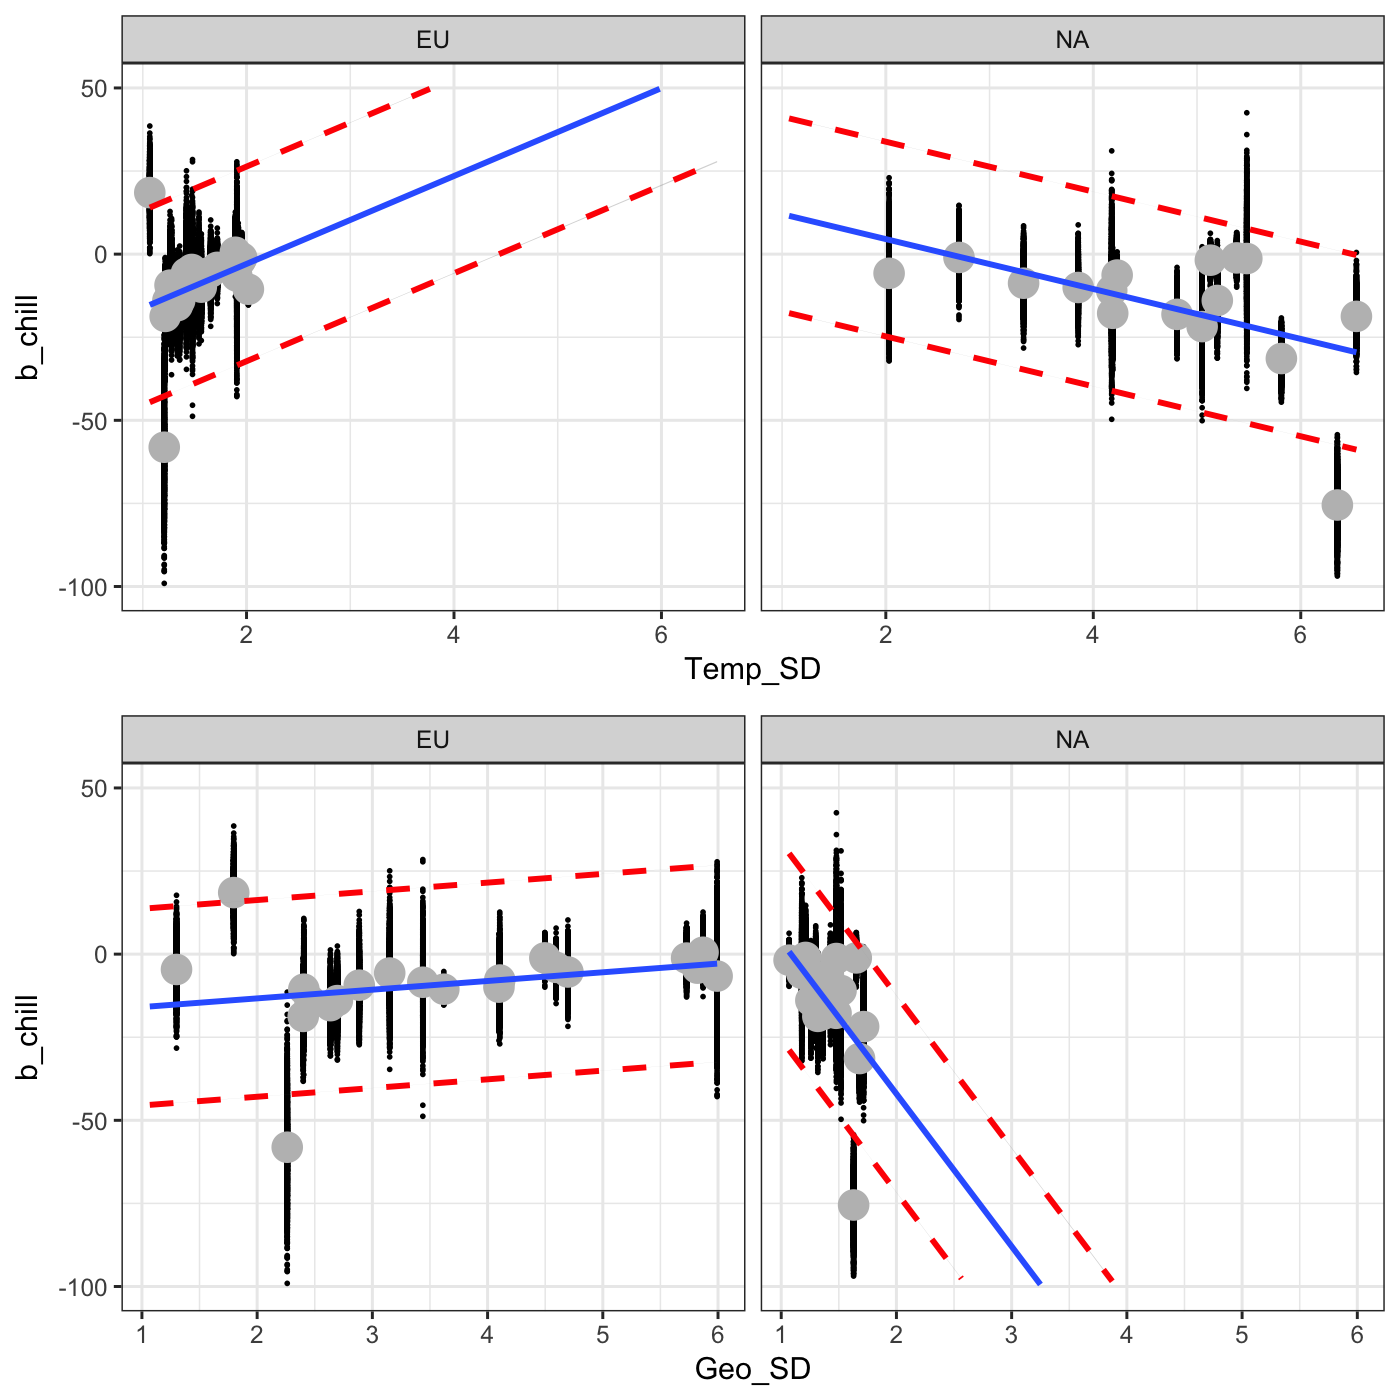
\includegraphics[width=0.6\textwidth]{..//..//figures/cheap_approach/modeled_stv.png}
    \caption{Influence of temporal and geographic variation in mean low temperature (stv) on $\beta_{chill}$. Model is pooling on iterations. Blue line is mean and red lines 95\% credible intervals} 
    \label{fig:stv}
\end{figure}

	}


	\frame{
		\frametitle{Hypothesis 4}
		\framesubtitle{Range margins drive chill or photoperiod sensitivity}

\begin{figure}[h!]
    \centering
         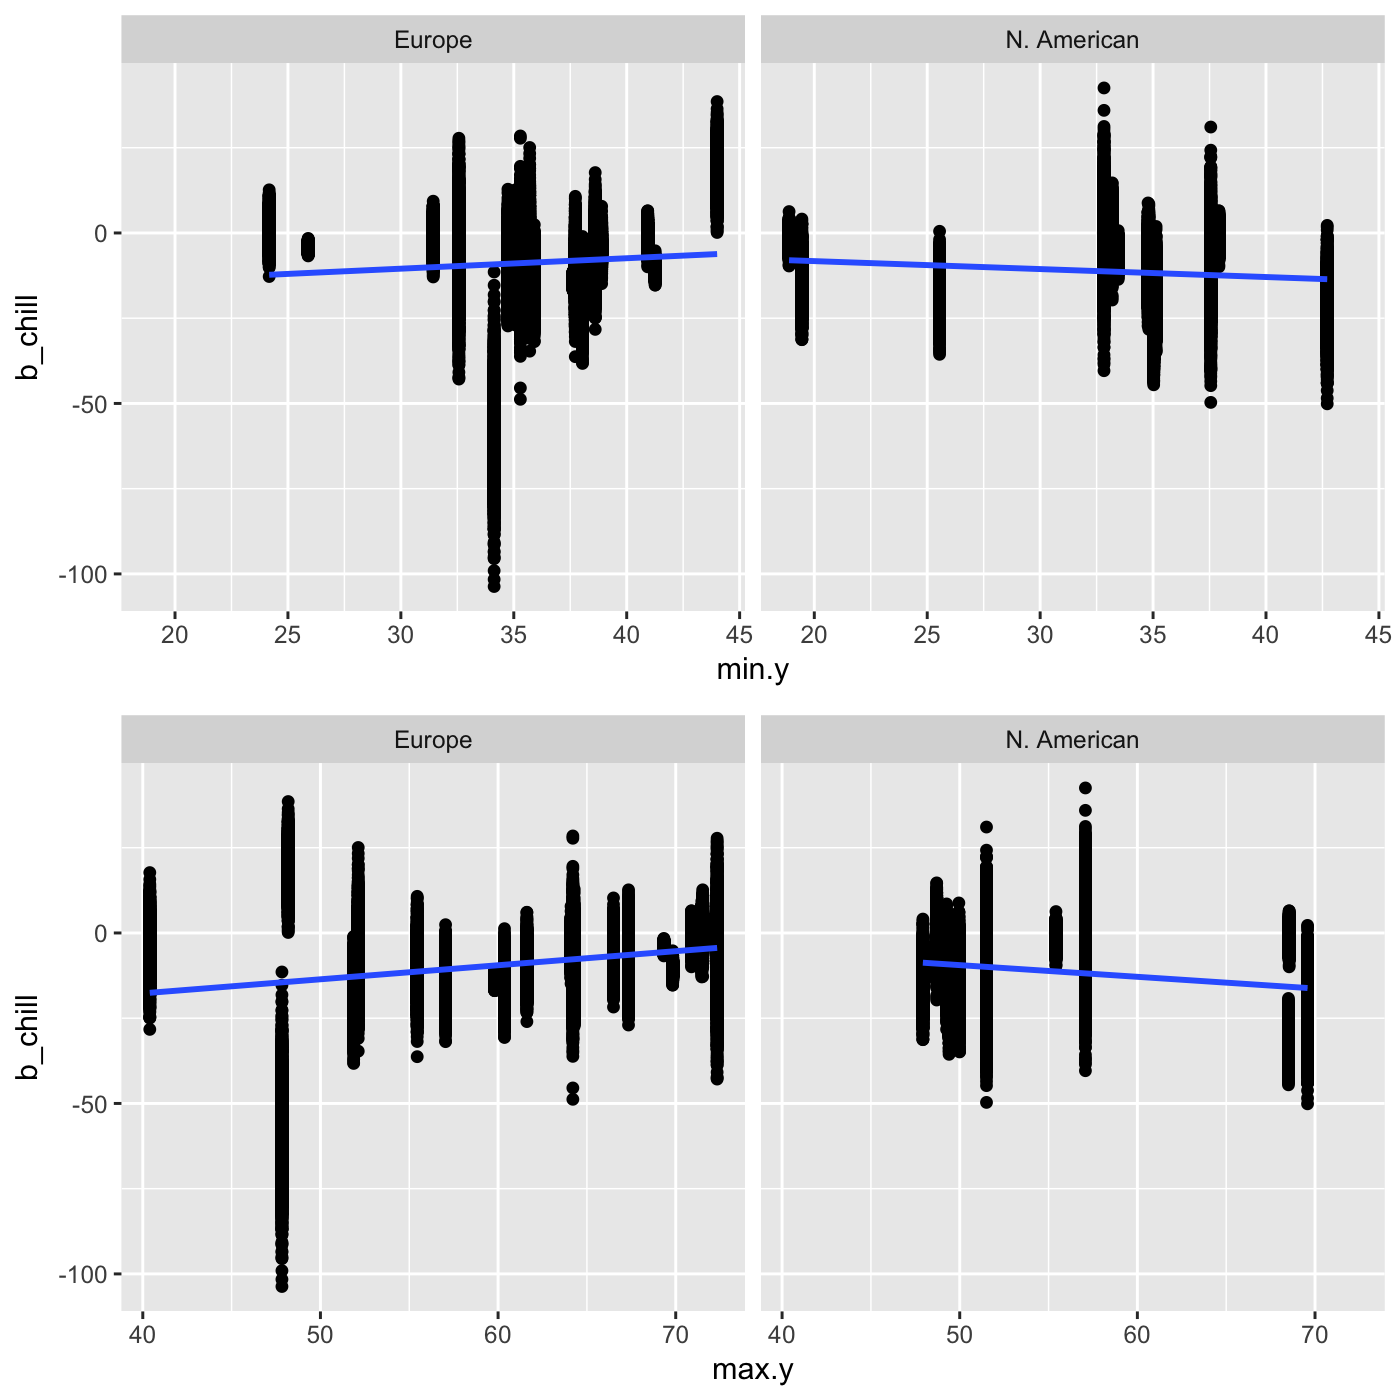
\includegraphics[width=0.6\textwidth]{..//..//figures/cheap_approach/unmodeled_lat.png}
    \caption{Influence of max. and min latitude. on $\beta_{chill}$. No hierarchy, simple linear model for now.} 
    \label{fig:lat}
\end{figure}

}

	\frame{
		\frametitle{Alternative hypotheses}
		\framesubtitle{In the future we will ...}
We don't see a lot of support for our hypothesis. Here are  some other ideas we are thinking of testing.
\begin{enumerate}
\item Intra-specific variation in cue use is high.
\item How much overlap there is in species' ranges drive cue use difference
\end{enumerate}

}

\frame{
		\frametitle{Intra-specific?}

We don't see a lot of support for ths hypothesis. \\

Inter-specific:\\
sd(force.z): 7.17\\    
sd(photo.z): 2.76  \\   

Intra-specific:\\

sd(force.z): 1.65 \\     
sd(photo.z): 0.62\\   


}

	\frame{
		\frametitle{New steps for the scientific community ...}
		\framesubtitle{To robustly deal with this ...}
		\begin{enumerate}
		\item Paleo-climate
		\item Better-data--- Phylogeny
		\item Community assembly--since we can't seperate leafout date from cue we should
		\end{enumerate}
}

	



{


\end{document}

\begin{figure}[h!]
\centering
\noindent \includegraphics[width=0.8\textwidth]{figures/brms_m1.png} 
\caption{No phylogenetic structure, just species on the intercept.}
\end{figure}

